\documentclass[]{article}
\usepackage{lmodern}
\usepackage{amssymb,amsmath}
\usepackage{ifxetex,ifluatex}
\usepackage{fixltx2e} % provides \textsubscript
\ifnum 0\ifxetex 1\fi\ifluatex 1\fi=0 % if pdftex
  \usepackage[T1]{fontenc}
  \usepackage[utf8]{inputenc}
\else % if luatex or xelatex
  \ifxetex
    \usepackage{mathspec}
    \usepackage{xltxtra,xunicode}
  \else
    \usepackage{fontspec}
  \fi
  \defaultfontfeatures{Mapping=tex-text,Scale=MatchLowercase}
  \newcommand{\euro}{€}
\fi
% use upquote if available, for straight quotes in verbatim environments
\IfFileExists{upquote.sty}{\usepackage{upquote}}{}
% use microtype if available
\IfFileExists{microtype.sty}{%
\usepackage{microtype}
\UseMicrotypeSet[protrusion]{basicmath} % disable protrusion for tt fonts
}{}
\usepackage[margin=1in]{geometry}
\usepackage{longtable,booktabs}
\usepackage{graphicx}
\makeatletter
\def\maxwidth{\ifdim\Gin@nat@width>\linewidth\linewidth\else\Gin@nat@width\fi}
\def\maxheight{\ifdim\Gin@nat@height>\textheight\textheight\else\Gin@nat@height\fi}
\makeatother
% Scale images if necessary, so that they will not overflow the page
% margins by default, and it is still possible to overwrite the defaults
% using explicit options in \includegraphics[width, height, ...]{}
\setkeys{Gin}{width=\maxwidth,height=\maxheight,keepaspectratio}
\ifxetex
  \usepackage[setpagesize=false, % page size defined by xetex
              unicode=false, % unicode breaks when used with xetex
              xetex]{hyperref}
\else
  \usepackage[unicode=true]{hyperref}
\fi
\hypersetup{breaklinks=true,
            bookmarks=true,
            pdfauthor={J.E. Turcotte},
            pdftitle={MPG Comparisons between Manual and Automatic Transmissions},
            colorlinks=true,
            citecolor=blue,
            urlcolor=blue,
            linkcolor=magenta,
            pdfborder={0 0 0}}
\urlstyle{same}  % don't use monospace font for urls
\setlength{\parindent}{0pt}
\setlength{\parskip}{6pt plus 2pt minus 1pt}
\setlength{\emergencystretch}{3em}  % prevent overfull lines
\setcounter{secnumdepth}{0}

%%% Use protect on footnotes to avoid problems with footnotes in titles
\let\rmarkdownfootnote\footnote%
\def\footnote{\protect\rmarkdownfootnote}

%%% Change title format to be more compact
\usepackage{titling}

% Create subtitle command for use in maketitle
\newcommand{\subtitle}[1]{
  \posttitle{
    \begin{center}\large#1\end{center}
    }
}

\setlength{\droptitle}{-2em}
  \title{MPG Comparisons between Manual and Automatic Transmissions}
  \pretitle{\vspace{\droptitle}\centering\huge}
  \posttitle{\par}
  \author{J.E. Turcotte}
  \preauthor{\centering\large\emph}
  \postauthor{\par}
  \predate{\centering\large\emph}
  \postdate{\par}
  \date{May 17, 2016}



\begin{document}

\maketitle


\subsection{Executive Summary}\label{executive-summary}

In this brief study, we must explore the effect that automatic versus
manual transmissions has over miles-per-gallon fuel efficiency among a
sample group of 1974 model automobiles.

\subsection{Assumptions}\label{assumptions}

\begin{itemize}
\itemsep1pt\parskip0pt\parsep0pt
\item
  The field `qsec' (or, from a stop, how many seconds it took for the
  vehicle to reach a quarter mile's distance) is likely a function of
  the car's power; i.e., a result, like miles per gallon, of the
  vehicle's configuration rather than a potential confounding cause OF
  miles per gallon. For that reason, I'm excluding it in any modelling
  of miles per gallon per vehicle.
\item
  Given the yes-or-no nature of whether or not a car is manufactured
  with or without automatic transmission, this data has been
  categorized, so named within the data, and is likely to be modelled
  using binomial logistic regression.
\end{itemize}

\subsection{Examining the Data}\label{examining-the-data}

Looking at \emph{Table 1}, we get a very quick sense of what the data
that we ahve to work with looks like. Given that not all these columns
(already exlcuding `vs' and `qsec') are easily read or in quite the
right format, the first step I've taken here is to rename the columns
and change the transmission data to a named factor.

Following this, \emph{Table 2} gives us a brief summarization of the
better-named data that remains, excluding a few extra columns for
brevity.

\subsection{Null Hypthothesis
(\(H_{0}\))}\label{null-hypthothesis-hux5f0}

\subsection{Alternative Hypothesis
(\(H_{a}\))}\label{alternative-hypothesis-hux5fa}

\subsection{Conclusion}\label{conclusion}

\subsection{Source}\label{source}

Henderson and Velleman (1981), \emph{Building multiple regression models
interactively}. Biometrics, 37, 391--411.

\subsection{Appendix}\label{appendix}

\subsubsection{Figure 1 - Some of the
data}\label{figure-1---some-of-the-data}

\begin{longtable}[c]{@{}lrrrrrrrrr@{}}
\toprule
& mpg & cyl & disp & hp & drat & wt & am & gear & carb\tabularnewline
\midrule
\endhead
Mazda RX4 & 21.0 & 6 & 160 & 110 & 3.90 & 2.620 & 1 & 4 &
4\tabularnewline
Mazda RX4 Wag & 21.0 & 6 & 160 & 110 & 3.90 & 2.875 & 1 & 4 &
4\tabularnewline
Datsun 710 & 22.8 & 4 & 108 & 93 & 3.85 & 2.320 & 1 & 4 &
1\tabularnewline
Hornet 4 Drive & 21.4 & 6 & 258 & 110 & 3.08 & 3.215 & 0 & 3 &
1\tabularnewline
Hornet Sportabout & 18.7 & 8 & 360 & 175 & 3.15 & 3.440 & 0 & 3 &
2\tabularnewline
Valiant & 18.1 & 6 & 225 & 105 & 2.76 & 3.460 & 0 & 3 & 1\tabularnewline
\bottomrule
\end{longtable}

\subsubsection{Figure 2 - Summary of data after
retitling}\label{figure-2---summary-of-data-after-retitling}

\begin{longtable}[c]{@{}lccccc@{}}
\toprule
& MPG & cylinders & horsepower & tons & manual\tabularnewline
\midrule
\endhead
& Min. :10.40 & Min. :4.000 & Min. : 52.0 & Min. :0.7565 & Min.
:0.0000\tabularnewline
& 1st Qu.:15.43 & 1st Qu.:4.000 & 1st Qu.: 96.5 & 1st Qu.:1.2906 & 1st
Qu.:0.0000\tabularnewline
& Median :19.20 & Median :6.000 & Median :123.0 & Median :1.6625 &
Median :0.0000\tabularnewline
& Mean :20.09 & Mean :6.188 & Mean :146.7 & Mean :1.6086 & Mean
:0.4062\tabularnewline
& 3rd Qu.:22.80 & 3rd Qu.:8.000 & 3rd Qu.:180.0 & 3rd Qu.:1.8050 & 3rd
Qu.:1.0000\tabularnewline
& Max. :33.90 & Max. :8.000 & Max. :335.0 & Max. :2.7120 & Max.
:1.0000\tabularnewline
\bottomrule
\end{longtable}

\subsubsection{Figure 3 - A simple bionomial
regression}\label{figure-3---a-simple-bionomial-regression}

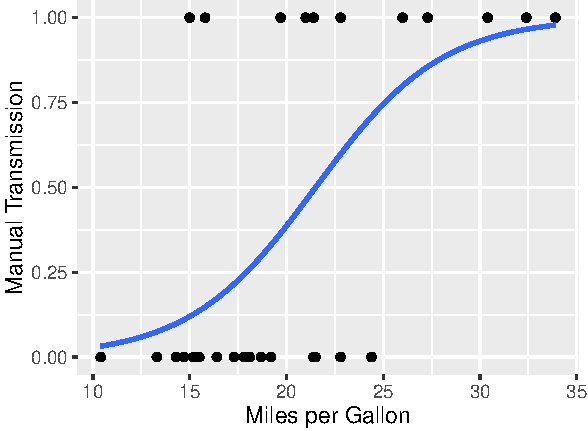
\includegraphics{study_files/figure-latex/simple binomial fit-1.pdf}

\end{document}
